   \documentclass[%
oneside,                 % oneside: electronic viewing, twoside: printing
final,                   % draft: marks overfull hboxes, figures with paths
10pt]{article}

\listfiles               %  print all files needed to compile this document

\usepackage[a4paper, total={6in, 8in}]{geometry}
\usepackage[totoc]{idxlayout}   % for index in the toc
\usepackage[nottoc]{tocbibind}  % for references/bibliography in the toc

\usepackage{relsize,makeidx,color,setspace,amsmath,amsfonts,amssymb}
\usepackage[table]{xcolor}
\usepackage{bm,ltablex,microtype}
\usepackage{comment} 
\usepackage[pdftex]{graphicx}

\usepackage{fancyvrb} % packages needed for verbatim environments

\usepackage[T1]{fontenc}
%\usepackage[latin1]{inputenc}
\usepackage{ucs}
\usepackage[utf8x]{inputenc}

%extra space in tabs
\usepackage{array}
\setlength{\extrarowheight}{.5ex}


\usepackage{lmodern}         % Latin Modern fonts derived from Computer Modern


\usepackage{pgfplotstable, booktabs}

\pgfplotstableset{
    every head row/.style={before row=\toprule,after row=\midrule},
    every last row/.style={after row=\bottomrule}
}


%Test subsubsubscetion
\usepackage{titlesec}
\usepackage{hyperref}

\titleclass{\subsubsubsection}{straight}[\subsection]

\newcounter{subsubsubsection}[subsubsection]
\renewcommand\thesubsubsubsection{\thesubsubsection.\arabic{subsubsubsection}}
\renewcommand\theparagraph{\thesubsubsubsection.\arabic{paragraph}} % optional; useful if paragraphs are to be numbered

\titleformat{\subsubsubsection}
  {\normalfont\normalsize\bfseries}{\thesubsubsubsection}{1em}{}
\titlespacing*{\subsubsubsection}
{0pt}{3.25ex plus 1ex minus .2ex}{1.5ex plus .2ex}

\makeatletter
\renewcommand\paragraph{\@startsection{paragraph}{5}{\z@}%
  {3.25ex \@plus1ex \@minus.2ex}%
  {-1em}%
  {\normalfont\normalsize\bfseries}}
\renewcommand\subparagraph{\@startsection{subparagraph}{6}{\parindent}%
  {3.25ex \@plus1ex \@minus .2ex}%
  {-1em}%
  {\normalfont\normalsize\bfseries}}
\def\toclevel@subsubsubsection{4}
\def\toclevel@paragraph{5}
\def\toclevel@paragraph{6}
\def\l@subsubsubsection{\@dottedtocline{4}{7em}{4em}}
\def\l@paragraph{\@dottedtocline{5}{10em}{5em}}
\def\l@subparagraph{\@dottedtocline{6}{14em}{6em}}
\makeatother

\setcounter{secnumdepth}{4}
\setcounter{tocdepth}{4}
%end of subsubsusbbu


% Hyperlinks in PDF:
\definecolor{linkcolor}{rgb}{0,0,0.4}
\usepackage{hyperref}
\hypersetup{
    breaklinks=true,
    colorlinks=true,
    linkcolor=linkcolor,
    urlcolor=linkcolor,
    citecolor=black,
    filecolor=black,
    %filecolor=blue,
    pdfmenubar=true,
    pdftoolbar=true,
    bookmarksdepth=3   % Uncomment (and tweak) for PDF bookmarks with more levels than the TOC
    }
%\hyperbaseurl{}   % hyperlinks are relative to this root

\setcounter{tocdepth}{2}  % levels in table of contents

% --- fancyhdr package for fancy headers ---
\usepackage{fancyhdr}
\fancyhf{} % sets both header and footer to nothing
\renewcommand{\headrulewidth}{0pt}
\fancyfoot[LE,RO]{\thepage}
% Ensure copyright on titlepage (article style) and chapter pages (book style)
\fancypagestyle{plain}{
  \fancyhf{}
  \fancyfoot[C]{{\footnotesize \copyright\ 1999-2018, "Computational Physics I FYS3150/FYS4150":"http://www.uio.no/studier/emner/matnat/fys/FYS3150/index-eng.html". Released under CC Attribution-NonCommercial 4.0 license}}
%  \renewcommand{\footrulewidth}{0mm}
  \renewcommand{\headrulewidth}{0mm}
}
% Ensure copyright on titlepages with \thispagestyle{empty}
\fancypagestyle{empty}{
  \fancyhf{}
  \fancyfoot[C]{{ }}
  \renewcommand{\footrulewidth}{0mm}
  \renewcommand{\headrulewidth}{0mm}
}

\pagestyle{fancy}


% prevent orhpans and widows
\clubpenalty = 10000
\widowpenalty = 10000

% --- end of standard preamble for documents ---


% insert custom LaTeX commands...

\raggedbottom
\makeindex
\usepackage[totoc]{idxlayout}   % for index in the toc
\usepackage[nottoc]{tocbibind}  % for references/bibliography in the toc
\usepackage{listings}
\usepackage[normalem]{ulem} 	%for tables
\useunder{\uline}{\ul}{}
\usepackage{hyperref}
\usepackage[section]{placeins} %force figs in section

\usepackage{natbib}

\usepackage[toc,page]{appendix} % appenix
\usepackage{amsmath} % split in align
\usepackage{multirow} %multirow


\usepackage{float}
\usepackage{subfig}


%-------------------- end preamble ----------------------

\begin{document}

% matching end for #ifdef PREAMBLE

\newcommand{\exercisesection}[1]{\subsection*{#1}}


% ------------------- main content ----------------------



% ----------------- title -------------------------

\thispagestyle{empty}

\begin{center}
{\LARGE\bf
\begin{spacing}{1.25}
BOLTZIEMANMACHINE YO!
\end{spacing}
}
\end{center}

% ----------------- author(s) -------------------------

\begin{center}
{\bf Johan Nereng}
\end{center}

    \begin{center}
% List of all institutions:
\centerline{{\small Department of Physics, University of Oslo, Norway}}
\end{center}
    
% ----------------- end author(s) -------------------------

% --- begin date ---
\begin{center}
Spring, 2020
\end{center}
% --- end date ---

\vspace{3cm}
\vspace{3cm}
\begin{abstract}
her kjem det greier
\end{abstract}


\newpage


\textit{\textbf{Author's comments:} HAdde en enorm motivasjonknekk midt i smesteret, og endte opp med å henge bakpå. takk for utvida frist, og igjen takk til Ø for masse god hjælp. Fant igjen motivasjonen med dette prosjektet - det var knallgøy! 
This was a blast! I found it really interesting to go into detail on my results. For once, I did not put that much effort into the theory section, and instead focused on interpreting the results. lalalala
I chose to mainly focus on examining results and discussing observations, rather than having a fleshed out theory section. As I have described the theory of neural networks, and VMC in other projects (in this course and FYS-STK), I found that I most of all wanted more experience in interpreting results.}
\newpage


\section{Introduction}



This is an extention paper to my previous project paper \textit{VMC: Effects of Importance Sampling and Jastrow factor on error estimates} \cite{JN_P1}, which is not published and not in review (not intended for publishing) \url{https://github.com/johanere/FYS4411/tree/master/Project\%201} . As such, this extention paper will not include descriptions of the theory already covered in \cite{JN_P1}. 

\paragraph{This project}introduces a new system, namely electrons in a harmonic oscillator, as such, the Hamiltonian of the system is changed from that of \cite{JN_P1}. As the state of the system is represented by a neural network quantum state(NQS), the trial wave function is also new. These two alterations result in a different expression for the local energy, and parameter gradients. In addition, this project introduces a new VMC sampling method, Gibbs sampling. 

As this is an extention paper, I will often reference the "orignail?" paaper, which in turns has relavnanat theory refkenmrken blalbal. USe some of the results from the orgina lpaper
method and the "automated blocking" algorithm from \citep{Jonsson}.

 Trene en RBM til å foreslå en god $\Psi$ slik at variational principle gir et godt estimat på $E_0$, det vil si lavest mulig - altså et tak. 
 
In order to write this project paper and the code required to produce the results, I used a variety of tools, including: C++, Python 3.7.7, NumPy \cite{numpy}, as well as a number of books, web-pages and articles - of which most are listed under 
 \hyperref[refer]{references}. All the code required to reproduce the results may be found on my \href{https://github.com/johanere/FYS4411}{github page }.  
\section{Material and methods} \label{theory}


\subsection{System: Electrons in 2D isotropic HO}
The system consists of $P$ electrons in a $D$ dimensional isotropic harmoinc oscillator (HO) potential, with the following idealized total Hamiltonian, when using natural units, ($\hbar=c=e=m_e=1$), and energies in  atomic units a.u:
\begin{equation}
\label{eq:finalH}
H=\sum_{i=1}^{P} \left(  -\frac{1}{2} \nabla_i^2 + \frac{1}{2} \omega^2r_i^2  \right)+\sum_{i=1}^P \sum_{j=1}^i \frac{1}{r_{ij}},
\end{equation}
Where $\omega$ is the oscillator frequency. 
\begin{equation*}
H_0=\sum_{i=1}^{P} \left(  -\frac{1}{2} \nabla_i^2 + \frac{1}{2} \omega^2r_i^2  \right),
\end{equation*}
is the standard HO part of the Hamiltonian, while
\begin{equation*}
H_1=\sum_{i<j}\frac{1}{r_{ij}},
\end{equation*}
is the interactive part, where $r_{ij}=\vert \bm{r}_1-\bm{r}_2\vert$, and $r_i = \sqrt{r_{i_x}^2+r_{i_y}^2}$.

\paragraph{The Pauli exlusion principle}requires that that two identical fermions, such as electrons, cannot occupy the same state \citep{Griffiths95}. As this project concerns itself with the ground state of a system of two non-interacting electrons, these electrons must therefore have opposite spins. This also means that the total spin of the two electron system in question must be zero, and that $P$ must be either one or two.

\paragraph{Analytic solutions}for the system are available, which makes evaluating the performance of the algorithms possible under certain caveats.  The energy of an harmonic oscillator is in one dimension is \citep{Griffiths95};

\begin{equation}
\begin{aligned}
E_n = \hbar \omega (n+\frac{1}{2}
\end{aligned}
\end{equation}

Thus, for a system of $P=\{1,2\}$ non-interacting electrons in $D$ dimensions,

\begin{equation}
\begin{aligned}
E_n = \hbar \omega (n+\frac{1}{2}
\end{aligned}
\end{equation}



\subsection{Neural network quantum state}
Instead of seeking to find suitable trial wave function ansatz for the system, this project represents the state of the system by a neural network quantum state (NQS), as was done in by Carleo and Troyer \citep{CarleoGiuseppe2017Stqm}. In their article, they suggest that one may view the wave function as a computational black box, which for a specific system configuration, outputs an amplitude corresponding to the value of the wave function. 

As was done in \citep{CarleoGiuseppe2017Stqm}, I've chosen to use a Restricted Boltzmann machine \cite{MLMurphy}[p.983] (RBM) when representing the state of the system. RBM models latent variables, or variables that are not directly observed, but rather inferred from other quantities - in this case, the local energy. The network consists of a layer of $M$ so called \textit{visible nodes}, and a layer of $N$ \textit{hidden nodes}. These layers have associated weights and biases, with a two-way feed forward. This enables the network both to output values for the hidden nodes as a function of the visible nodes, and vice versa. This means that an RBM is a generative model, in this case a model which can generate particle positions from a distribution. This distribution is a function of the weights and biases, as well as the hidden nodes. 


\paragraph{The marginal probability of the network} is given by
\begin{equation*}
\begin{aligned}
F_{rbm}(\bm X) = \frac{1}{Z} \sum_h e^{-E(\bm X, \bm h} ,
\end{aligned}
\label{eq:TWF}
\end{equation*}



and corresponds to the probability of the system state, $\bm X$. As $\bm X$ in this case is a vector of continuous particle positions, the energy function, $E(\bm X, \bm h)$ of the network (not to be confused with the energy of the system), must be defined accordingly. There are various forms of RBMs with different energy functions, specialized to different types of data. The one used here, which enables continous $\bm X$, is known as a \textit{Gaussian-Binary RBM} \cite{MLMurphy}[p.986], and also includes binary hidden nodes $\bm H=\{h_j\}$ for $j=1,2,..,N$, and $h_j \in \{0,1\}$. Using it's associated energy function, and representing each particle position as $X_i$, such that $i=1,2,..,M$ where $M=PD$, results in the following NQS/wave form representation \cite{MLoppgave}; 

\begin{equation}
\begin{aligned}
\Psi (\mathbf{X}) &= F_{rbm}(\mathbf{X}) \\
&= \frac{1}{Z} \sum_{\{h_j\}} e^{-\sum_i^M \frac{(X_i - a_i)^2}{2\sigma^2} + \sum_j^N b_j h_j + \sum_{i,j}^{M,N} \frac{X_i w_{ij} h_j}{\sigma^2}} \\
&= \frac{1}{Z} e^{-\sum_i^M \frac{(X_i - a_i)^2}{2\sigma^2}} \prod_j^N (1 + e^{ v(j)}) \\
\end{aligned}
\end{equation}
\begin{equation}
\begin{aligned}
v(j) = b_j + \sum_{i=1}^M \frac{X_i W_{ij} }{\sigma^2}
\end{aligned}
\label{eq:v_j}
\end{equation}

Since all evaluations of the wave function is in the context of finding a ratio of probabilities; $\frac{\Psi_{rbm}^{new}}{\Psi_{rbm}^{old}}$, and all other quantities are derivatives of $\ln \Psi_{rbm}$, the normalization constant $Z$ is not relevant.


\subsubsection{Local Energy and drift force}
As described in project 1 \cite{JN_P1}[2.2], the results obtained through the VMC methods used in this project relies on the variational principle. As such, the local energy
\begin{equation}
    E_L(\mathbf{r})=\frac{1}{\Psi_T(\mathbf{r})}H\Psi_T(\mathbf{r}).
    \label{eq:locale}
 \end{equation}
is required in order to carry out the Monte Carlo integration for the ground state energy. Using the trial wave function \eqref{eq:TWF}, and \eqref{eq:locale} an analytic expression for the local energy may be fond. This is derived in detail in \hyperref[APP_1]{Appendix 1: Analytic expression for the local energy}, and will not be discussed further here. Based on the same appendix, the correponding drift force, needed for the importance sampling \cite{JN_P1}[2.2.2], is;

\begin{equation}
F_i = \frac{2\nabla \Psi_T}{\Psi_T} = 2 \left[- \frac{(X_k - a_k)}{\sigma^2} + \sum_{i}^N \frac{w_{kj}}{\sigma^2}\frac{1}{1 + e^{-v(\bm X,j)}} \right]
\end{equation} 

\subsection{Updating parameters}
As the weights of the RBM are initialized randomly, the resulting energy is unlikely be the best approximation the algorithm is capable of. In \cite{JN_P1}, the aim was to find $\alpha$ s.t the energy was minimized. Here, the aim is instead to optimize the network.  This is done by optimizing the weights $\bm X$, and biases $\bm a$ and $\bm b$, using the energy as a cost function. Although this optimization is over multiple parameters of different types, the strategy for each parameter $\beta_i$ of parameter type $\beta$, which can either be $\bm a$, $\bm b$, or $\bm X$, is the same as for $\alpha$ described in more detail in \cite{JN_P1}[2.2.3]. The update scheme for parameter $\beta$ is;
\begin{equation}
\bm{\beta}_{k+1}=\bm{\beta}_{k}-\eta_k  \bm g (\bm{\beta}_k),
\label{eq:GD_beta}
\end{equation}
where $\eta$ is the learning rate. \eqref{eq:GD_beta} requires the gradient of the local energy w.r.t the parameters in $\bm \beta$, $\bm g (\bm \beta)=\nabla_{\beta} \langle E_L \rangle$. This is given by

\begin{align*}
\nabla_{\beta} \langle E_L \rangle = 2 \left( \langle \frac{\bar \Psi_{\beta}}{\Psi [\beta]} E_L[\beta] \rangle - \langle \frac{\bar \Psi_{\beta}}{\Psi [\beta]} \rangle \langle E_L[\beta] \rangle  \right),
\end{align*}

where $\frac{\bar \Psi_{\beta}}{\Psi [\beta]} = \frac{1}{\Psi_{rbm,\beta} } \frac{\partial \Psi_{rbm,\beta}}{\partial \beta}$. Expressions for $\beta = a,b,W$ can be found in \hyperref[APP_2]{Appendix 2: Derivatives w.r.t RBM parameters}.

\subsection{Gibbs Sampling}
Gibbs sampling \cite{MLMurphy}[ch.24.2] is a Markov Chain Monte Carlo (MCMC) algorithm, analogous to coordinate descent in an MCMC framework. In this implementation, the two-way feed forward network, the RBM, is used to sample the joint probability of $\bm X$ and bm $\bm H$ in a two step process. First, $P(\bm H|\bm X)$ is used to determine the state of the binary nodes $ H$, for the current system state $\bm X$. Then, after having updated $\bm H$, $P(\bm X|\bm H)$ is used to sample a new system state. In contrast to the Metropolis Hastings algorithm, the probability of accepting this proposed system state equals one \cite{Flugsrud}, ie. every proposal is accepted. The conditional probabilities are given by;
\begin{equation}
\begin{aligned}
P(H_j=1|\bm X) & = \frac{1}{1+e^{-b_j-\sum_i^M \frac{X_i W_{ij}}{\sigma^2}}}=\text{logistic} (-(v(j)) \\
P(H_j=0|\bm X) & =\text{logistic} ((v(j)) \\
\end{aligned}
\label{eq:gibbs_prob_h}
\end{equation}

and

\begin{equation}
\begin{aligned}
P(X_i|\bm H) = \mathcal{N} (X_i;a_i+\bm W_{i*}\bm H,\sigma^2) 
\end{aligned}
\label{eq:gibbs_prob_x}
\end{equation}

In order to sample $\Psi_{T,Gibbs}(\bm X)$ s.t $\vert \Psi_{T,Gibbs}(\bm X) \vert^2$ can be interpreted as a probability, $\Psi_{T,Gibbs}(\bm X)=\sqrt{F_{rbm}(\bm X)}$, under the assumption that the wave function is positive definite. This slightly changes the expressions the local energy and parameter gradients, as is described briefly in \hyperref[APP_3]{Appendix 3: Local energy and parameter gradients for Gibbs sampling}. 

Having an acceptance rate of $1$ means that the Gibbs algorithm should have a short burn-in phase (see the Implementation sub chapter). Given sufficient training, I also expect this method to have a smaller estimation error. 

\subsection{Implementation} 
I have chosen to structure my code s.t. a single experiment uses a single RBM object. This RBM object owns a set of weights and biases, which it updates after each Monte Carlo simulation. In each Monte Carlo simulation, I construct a system object, which holds information about the system, and which calls on a sampler object that samples the energy as well as relevant quantities for calculating the gradient of the parameters. 

In each Monte Carlo simulation, I intend to discard all samples in an initial \textit{burn-in phase} \citep{MLMurphy}[p.856], or equilibrium phase, \citep{MLMurphy}[p.856], as is common practice when using VMC methods. The effective length of this burn-in phase will be decided in the initial tests of the system, and is intended to suit the simulation length as well as other practicalities, such as the error analysis.

For the two Metropolis Hastings algorithm, the brute force approach and the Importance Sampling approach, I use the algorithm in \cite{JN_P1}[2.2.1], with the local energy expression derived in appendix 1. This algorithm explicitly covers the brute force approach, but the changes needed to use the algorithm for Importance Sampling is explained in \cite{JN_P1}[2.2.2]. As the RBM does not inherently distinguish between particles, I chose to treat each position coordinate as a visible node. In each update step of the Metropolis Hastings methods, I therefor only change the value of a single visible node, instead of moving an entire particle. In the case of Gibbs sampling, all particle positions are sampled at each MC cycle. The energy contribution from the interacting term of the Hamiltonian is the only quantity which directly distinguishes between particles, and is therefor implemented in a way that ensures this. 
 
\subsubsection{Algorithm}
The following algorithm gives an overview of the operations in a single experiment;
\begin{center}\fbox{\parbox{\textwidth}{{\textbf{Algorithm: VMC using RBM with parameter optimization }}
\begin{enumerate}
\item Initialize algorithm
\subitem - Set number of iterations, $G$
\subitem - Set the number of Monte Carlo cycles, $MC$, and "burn in fraction".
\subitem - Set VMC method
\subsubitem - Set expression for $E_L$ and $\frac{\bar \Psi_{\beta}}{\Psi [\beta]}$ according to choice of method
\subsubitem - If using a variant of the Metropolis Algorithm, set step length, $l$
\subitem - Initialize RBM parameters $\bm a = \mathcal{U}(0,1/M), \bm b = \mathcal{U}(0,1/N),\bm W=\mathcal{U}(0,1/(M\times N)$ 
\item Execute Monte Carlo scheme
\subitem - Initialize visible nodes, $\bm X= \mathcal{U}(-1,1) $, set $E=0$ 
\subitem - For $cycle=1,2,..,MC$
\subsubitem - Propose new configuration according to VMC method
\subsubitem - Evaluate proposal, reject or accept. 
\subsubitem - If $cycle\geq MC \times$ "burn in fraction", calculate $E_L$ using current state.
\item Calculate $\langle H \rangle = \frac{E}{M}$
\item Optimize parameters $\bm a, \bm b, \bm W$ 
\item If the number of iterations of step $2$ is less than $G$, go to step 2. Else, end simulation
\end{enumerate}}}\end{center}


\subsection{Error analysis}
In \cite{JN_P1} I found that the error estimate, $\sigma$, on correlated data without methods such as "blocking" is large deceptive. Hence, I have chosen to exclusively use the standard error (error estimate using "blocking"), $\hat \sigma$ in this project. This means that the error analysis of this extension paper is similar to the error analysis of project paper one. For the sake of clarity, I would like to stress that when using $\hat \sigma$ I am referring to the standard error of the energy estimate $\bar E$, and when I am using $ \sigma$ is am referring to standard deviation of the probability distribution of the RBM.

\section{Results} \label{results}
In the following examinations I will not be using the interacting Hamiltonian. Interacting in VMC and RBM is studied in some detail later.
\subsection{Initial testing of VMC methods}
In order to ascertain whether or not the implementation of the various VMC methods were successful, I ran an MC simulation over $2^{21}$ cycles $P=1$, $D=1$, $N=2$, using Brute Force ($l=1.0$), Importance Sampling ($\Delta t=1.0$), and Gibbs Sampling. 

Figure \ref{fig:inital_1} shows the estimated energy $\bar E$ (left), and the absolute difference between the estimated energy at each cycle $\bar E(cycle)s$ and final estimated energy $\bar E$ (right), using the same seed for all three simulations. $\bar E$ is, as may be expected from an untrained network, relatively far from the exact energy. It is however clear that all three methods find a more-or-less stable value for $\bar E$ after a burn-in phase.  Similarly stable $\bar E$ values after burn-in was observed in subsequent tests using different seeds. As such, the VMC methods are deemed successfully implemented.
	\begin{figure}
		\centering
		\subfloat[Energy estimate]{{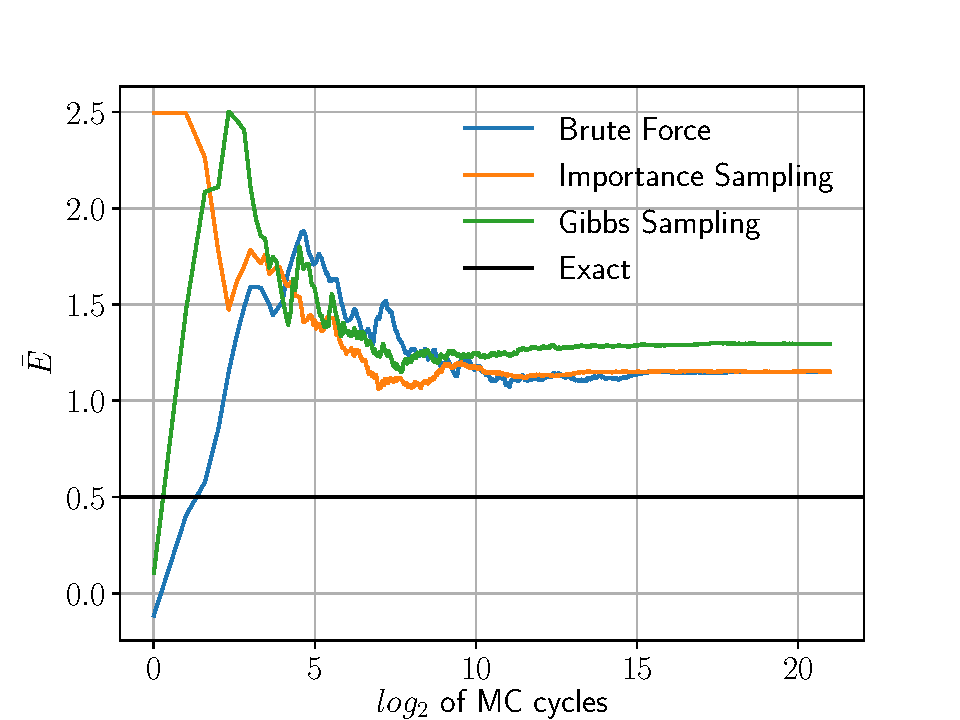
\includegraphics[width=8cm]{../Results/sim_0/initial_energies.pdf}}}
		\subfloat[Difference in energy estimate from final estimate]{{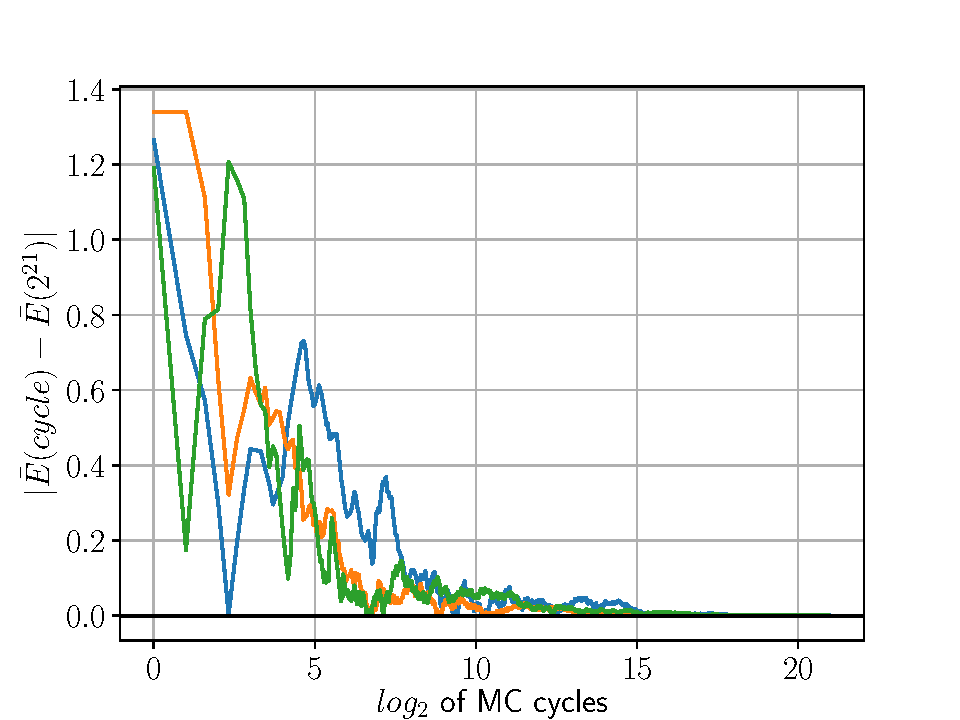
\includegraphics[width=8cm]{../Results/sim_0/initial_energies_abs.pdf}}}
		\caption{Initial test of the three VMC methods (same seed)}
		   \label{fig:inital_1}   
	\end{figure}


\subsection{Standard simulation settings}
Based on trial and error when initially testing the networks, I came to the conclusion that $2^{21}$ MC cycles give sufficient convergence to illuminate the qualities of the model. As such, I will use $2^{21}$ cycles unless otherwise stated.

As the blocking method requires data of a length which is a power of $2$, I will henceforth discard all samples taken in the first half of the MC cycles (as I run cycles in powers of 2). This should (more than) ensure that samples in the burn-in phase is discarded, as well as provide a suitable data format for the automated blocking method. 

Having established that the three VMC methods are capable of achieving energy convergence, I did a survey of the effects of $l$ (BF) and $\Delta t$ (IS).  I averaged $12$ experiments, each using $7$ optimization runs, and evaluating the results of the 8'th run by $\hat \sigma$. From the results presented in \hyperref[APP_4]{Appendix 4: Testing step length $l$ and $\Delta t$}, in figures
\ref{fig:app_4_IS} and  \ref{fig:app_4_BF}, I conclude that $l=1.0$ (BF) and $\Delta t=2.0$ are suitable parameters, and will use those values in subsequent experiments, unless otherwise stated.
\subsection{Comparison of Metropolis Hastings algorithms in training and RBM, n=2}
Before directly comparing the methods, I wanted to find a suitable range of values for $\eta$ to test the methods on. As such, I used $10$ values of $\eta=[0.1,1.0]$.  Figure \ref{fig:training_BF} and  \ref{fig:training_IS} in \hyperref[APP_4]{Appendix 4: Testing learning rate $\eta$}, show the results after the least suitable values of $\eta$ were discarded IOT clean up the figures. Cross checking the two plots, I found that $\eta=[0.3,0.4]$ was the only two adjacent values (with $\Delta =0.1)$ which were both within $10^{-3}$ of $\bar E$ for both methods. The figures also show that for $\eta=[0.3,0.4]$,  $\bar E-0.5<10^{-4}$ for all training iterations $\geq 10$, indicating a minima of the cost function, which I judge to mean that the RBM is "sufficiently trained". 

\subsubsection{Focused examination of training RBMs using Metropolis Hastings algorithms} \label{Results_focused_MH}
Next, I wanted to simultaneously compare BF and IS, and zero in on the best suited learning rate $\eta$. As $\hat \sigma$, measures the variance of the samples adjusted for correlation, ie. variance of the underlying sample distribution, I also needed an evaluation metric that reflected how close $\bar E$ was to the analytic $E=0.5$. For this, I chose to use the squared difference between estimated energy, $\bar E$ and $E=0.5$, $(\Delta E)^2$. 

I averaged $\hat \sigma$ and $(\Delta E)^2$ in each experiment for each $\eta$ after $10$ training iterations, over the next $5$ training iterations. Smaller values of mean $(\Delta E)^2$ indicate that the loss function is sufficiently minimized, while smaller values of  $\hat \sigma$ indicate that the network is estimating consistently.  As such, the best suited $\eta$ should produce the smallest  $(\Delta E)^2$,  and a sufficiently small $\hat \sigma$. In order to average out noise, I repeated the experiments $15$ times using different seeds and averaged the results, which are shown in table \ref{table:BF_IS_eta}. I included experiments for IS using $\Delta t=1.0$ so that I could validate my previous findings on the choice of time step.

\begin{table}[h!]
\begin{center}
\begin{tabular}{l|l|l|l|l|l|l} \hline
\multirow{2}{*}{\begin{tabular}{c} $\eta	$ \end{tabular}} & \multicolumn{2}{c|}{BF} &\multicolumn{2}{c|}{IS $\Delta t=1.0$} & \multicolumn{2}{c}{IS $\Delta t=2.0$} \\ \cline{2-7}
	    			& Mean $(\Delta E)^2$ 		& Mean $\hat \sigma$	& Mean $(\Delta E)^2$		& Mean $\hat \sigma$	&Mean $(\Delta E)^2$ 			& Mean $\hat \sigma$		\\ \hline 
$ 0.26 $ &  $ 1.04\times 10^{-4 } $ & $ 2.66\times 10^{-8 } $ & $ 4.92\times 10^{-5 } $ & $ 2.09\times 10^{-8 } $ & $ 8.33\times 10^{-5 } $ & $ 2.62\times 10^{-8 } $  \\
$ 0.28 $ &  $ 1.08\times 10^{-4 } $ & $ 4.33\times 10^{-8 } $ & $ 5.09\times 10^{-5 } $ & $ 4.43\times 10^{-8 } $ & $ 8.62\times 10^{-5 } $ & $ 4.79\times 10^{-8 } $  \\
$ 0.30 $ &  $ 1.05\times 10^{-4 } $ & $ 5.32\times 10^{-8 } $ & $ 4.96\times 10^{-5 } $ & $ 5.78\times 10^{-8 } $ & $ 8.50\times 10^{-5 } $ & $ 6.07\times 10^{-8 } $  \\
$ 0.32 $ &  $ 1.01\times 10^{-4 } $ & $ 6.00\times 10^{-8 } $ & $ 4.80\times 10^{-5 } $ & $ 7.90\times 10^{-8 } $ & $ 8.12\times 10^{-5 } $ & $ 7.80\times 10^{-8 } $  \\
$ 0.34 $ &  $ 1.09\times 10^{-4 } $ & $ 6.85\times 10^{-8 } $ & $ 5.16\times 10^{-5 } $ & $ 6.79\times 10^{-8 } $ & $ 8.70\times 10^{-5 } $ & $ 7.11\times 10^{-8 } $  \\
$ 0.36 $ &  $ 5.43\times 10^{-5 } $ & $ 4.58\times 10^{-9 } $ & $ 2.60\times 10^{-5 } $ & $ 4.10\times 10^{-9 } $ & $ 4.42\times 10^{-5 } $ & $ 4.81\times 10^{-9 } $  \\
$ 0.38 $ &  $ 8.70\times 10^{-5 } $ & $ 1.69\times 10^{-8 } $ & $ 4.14\times 10^{-5 } $ & $ 1.78\times 10^{-8 } $ & $ 7.09\times 10^{-5 } $ & $ 1.66\times 10^{-8 } $  \\
$ 0.40 $ &  $ 8.52\times 10^{-5 } $ & $ 7.28\times 10^{-9 } $ & $ 4.05\times 10^{-5 } $ & $ 6.45\times 10^{-9 } $ & $ 6.94\times 10^{-5 } $ & $ 7.00\times 10^{-9 } $  \\
$ 0.42 $ &  $ 1.11\times 10^{-4 } $ & $ 4.05\times 10^{-8 } $ & $ 5.26\times 10^{-5 } $ & $ 3.39\times 10^{-8 } $ & $ 8.92\times 10^{-5 } $ & $ 3.46\times 10^{-8 } $  \\
$ 0.44 $ &  $ 1.20\times 10^{-4 } $ & $ 1.87\times 10^{-7 } $ & $ 5.63\times 10^{-5 } $ & $ 1.48\times 10^{-7 } $ & $ 9.54\times 10^{-5 } $ & $ 1.47\times 10^{-7 } $  \\
  \\
 \hline
\end{tabular}
\end{center}
\caption{Comparison of methods: squared difference between estimated energy, $\bar E$ and $E=0.5$, $(\Delta E)^2$, and standard error using blocking, $\hat \sigma$, averaged over gradient descent iterations $10,11,12,13,14,15$, which are again averaged over $15$ experiments for different learning rates $\eta$.}
\label{table:BF_IS_eta}
\end{table}

Table \ref{table:BF_IS_eta} shows that for the Brute Force method, mean $(\Delta E)^2$ ranges from $\sim 10^{-4}$ to $\sim 10^{-5}$ for different values of $\eta$. $\eta=0.36,0.38, 0.40$ give the best average $(\Delta E)^2 \sim 10^{-5}$. Mean $\hat \sigma$ ranges from $\sim 10^{-8}$ to $\sim 10^{-9}$. For BF ($l=1.0$), $\eta=0.40$ appear to give both the lowest $(\Delta E)^2 (\sim 10^{-5})$ and the lowest $\hat \sigma$ ($\sim 10^{-9})$. 

All values of  $(\Delta E)^2$ is $\sim 10^{-5}$ for both choices of $\Delta t$ when using IS, while $\hat \sigma$ is similar for all values of $\eta$ across both BF and the two tested cases of IS. 
Comparing IS $\Delta t=1.0$ and $\Delta t=2.0$ clearly indicates that $\Delta t=2.0$ is better suited, as all values of $(\Delta E)^2$ are twice as high in the $\Delta t=1.0$ case, strengthening the validity of initially choosing $\Delta t=2.0$.

For IS $\Delta t=2.0$, $(\Delta E)^2$ is lowest for $\eta=0.34$, albeit at $\hat \sigma\sim 10^{-8}$. Hence, I conclude that $\eta = 0.34$ is the best suited for IS (with $\Delta t=2.0)$.

As all values of $(\Delta E)^2$ was $\sim 10^{-5}$ for IS, compared to $\sim 10^{-4}$ to $\sim 10^{-5}$ depending on $\eta$ for BF, I conclude that when using an RBM, BF is more sensitive than IS to the choice of learning rate w.r.t accuracy of energy estimates. I furthermore conclude that the effects of $\eta$  on $\hat \sigma$ is the same for both BF and IS, regardless of the value of $\Delta t$. 
When using the optimal $\eta$ values based on $(\Delta E)^2$ alone, BF and IS performed equally well, producing $(\Delta E)^2 \approx 8.7 \times 10^{-8}$ with $\hat \sigma = 7 \times 10^{-8}$, when averaged over 15 experiments.

\subsection{Gibbs Sampling, n=2}
As GS samples positions from a distribution (\eqref{eq:gibbs_prob_x}), the standard deviation of that distribution, $\sigma$, directly influences the state of the system, and hence also the energy. In the initial test of VMC methods shown in figure \ref{fig:inital_1}, it is clear that the two Metropolis Hastings methods converged to a different $\bar E$ than the Gibbs Sampler (GS). This offset in convergence for GS is likely the result of it's direct dependence on $\sigma$. As such, I ran $8$ experiments ($\eta=0.3$) with $\sigma$ ranging from $0.65$ to $1.0$, and plotted the results (see \hyperref[APP_4]{Appendix 4: Testing $\sigma$ for GS}) From figure \ref{GS_sigma_initial}, it is clear that the value of $\sigma$ influences $\bar E$, as expected. For $P=D=1$, $n=2$ it appears that the correct value of $\sigma$ lies somewhere between $0.9$ and $0.95$. In order to narrow down the value of $\sigma$ further, I ran $8$ experiments using $\sigma=[0.9,0.935]$.
 
Figure \ref{fig:inital_1} shows $\bar E$ for $\sigma=[0.9,0.935]$. It is clear that $\bar E$ converges after few iterations compared to BF and IS (see figures in \hyperref[APP_4]{Appendix 4}). Where $\bar E$ from BF and IS fluctuate (although marginally after $\sim 10$ iterations) for all tested $\eta$ values across all iterations, $\bar E$ reaches a stable value after $\sim 8$. This indicates that the RBM is either fully trained, or training very slow (relative to BF and IS), when using $\eta$ of the same magnitude $\sim 0.3$. Judging by the trajectories of $\bar E$ for the different values of $\sigma$, it also appears that $\bar E$, after $\sim 6$  iterations, may be moved arbitrarily close to $E=0.5$ by adjusting $\sigma$. 
\begin{figure}[!h]
        \centering 
         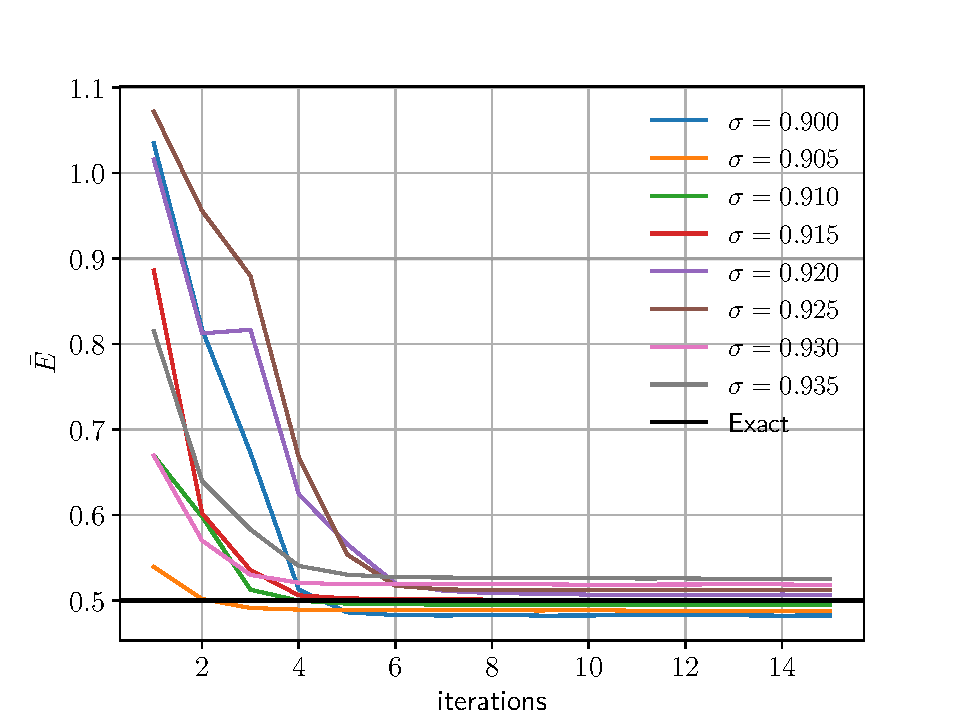
\includegraphics[scale=0.8]{../Results/sim_8/GS_sigma.pdf} 
        \caption{Gibbs Sampling:  $\bar E$ for different values of $\sigma$ }
        \label{fig:GS_sigma}   
\end{figure}  


\subsubsection{Focused examination of training RBMs using Gibbs Sampling} \label{Results_focused_GS}
When producing the results presented in figure \ref{fig:inital_1}, $\eta = 0.3$ was used. This value was picked arbitrarily for testing the effects of $\sigma$. In order to obtain a better suited value of $\eta$, I ran an experiment for a wide range of $\eta$ values. Based on the results (shown in figure \ref{fig:GS_eta} in \hyperref[APP_4]{Appendix 4}) I chose to do a closer examination of $\eta$ between $0.22$ and $0.38$ in increments of $0.2$. I ran a simulation for each value, averaging $(\Delta E)^2$ and $\hat \sigma$ as in the \hyperref[Results_focused_MH]{focused examination of training RBMs using Metropolis Hastings algorithms}, the results of which are in table \ref{table:GD_eta}. 

Table \ref{table:GD_eta} shows that $(\Delta E)^2$ between $\sim 10^{-5}$ and $\sim 10^{-6}$, $\sigma$ is $\approx 1.4 \times 10^{-3}$ , for all tested values of $\eta$. $\eta=0.26$ has the lowest $(\Delta E)^2$ ( $8.41 \times 10^{-6} $), and is therefor deemed as the best suited value among the ones that were tested. 

Comparing the best values of $(\Delta E)^2$ from BF($\approx 8.70\times 10^{-5 }$), IS ($\approx 8.62\times 10^{-5 }$), and GS ($\approx 8.41\times 10^{ -6 }$), indicates that $GS$ approximates $E$ for $P=D=1$ with $n=2$. However, the associated $\hat \sigma$ was $\sim 10^{-3}$ for GS, compared to $\sim 10^{-8}$ for BF and IS. This means that in the case of GS, the energy samples fluctuate (comparatively) wildly, around mean which is  (comparatively) close to the exact energy. BF and IS on the other hand exhibit a lot smaller fluctuations around a mean which is further from the exact energy.  Because of this, $\bar E$ should be sampled for a longer time when using GS, than what is necessary when using BF or IS. 

\begin{table}[h!]
\begin{center}
\begin{tabular}{lll}
\hline
 $\eta$ & Mean $(\Delta E)^2$ & Mean $\hat \sigma$ \\
\hline
$ 0.22 $ &  $ 7.17\times 10^{ -6 } $ & $ 1.40\times 10^{ -3 } $  \\
$ 0.24 $ &  $ 2.21\times 10^{ -5 } $ & $ 1.41\times 10^{ -3 } $  \\
$ 0.26 $ &  $ 8.41\times 10^{ -6 } $ & $ 1.40\times 10^{ -3 } $  \\
$ 0.28 $ &  $ 6.07\times 10^{ -6 } $ & $ 1.40\times 10^{ -3 } $  \\
$ 0.30 $ &  $ 1.76\times 10^{ -5 } $ & $ 1.41\times 10^{ -3 } $  \\
$ 0.32 $ &  $ 6.95\times 10^{ -6 } $ & $ 1.40\times 10^{ -3 } $  \\
$ 0.34 $ &  $ 5.35\times 10^{ -6 } $ & $ 1.40\times 10^{ -3 } $  \\
$ 0.36 $ &  $ 1.35\times 10^{ -5 } $ & $ 1.41\times 10^{ -3 } $  \\

\hline
\end{tabular}
\end{center}
\caption{Gibbs Sampling: squared difference between estimated energy, $\bar E$ and $E=0.5$, $(\Delta E)^2$, and standard error using blocking, $\hat \sigma$, averaged over gradient descent iterations $10,11,12,13,14,15$, which are again averaged over $15$ experiments for different learning rates $\eta$.}
\label{table:GD_eta}
\end{table}


\subsection{Comparison of VMC methods: 2 interacting electrons, n=4}
I ran experiments for each of the three methods, using values of $\eta, \sigma, l, \Delta t$ from table \ref{table:sim_set}, for $20$ optimization iterations, repeated $10$ times. 
\begin{table}[h!]
\begin{center}
\begin{tabular}{llll}
\hline
Method & $\eta$ & $\sigma$ & Step length \\
\hline
BF &  $ 0.38 $  & $ 1.0$ & $l=1.0$  \\
IS &  $ 0.34 $  &$1.0 $  & $\Delta t=2.0$\\
GS &  $ 0.26 $ &$0.914 $ & -  \\
\hline
\end{tabular}
\end{center}
\caption{Comparison of VMC methods: Linear Regression fit}
\label{table:sim_set}
\end{table}

\begin{figure}[!h]
        \centering 
         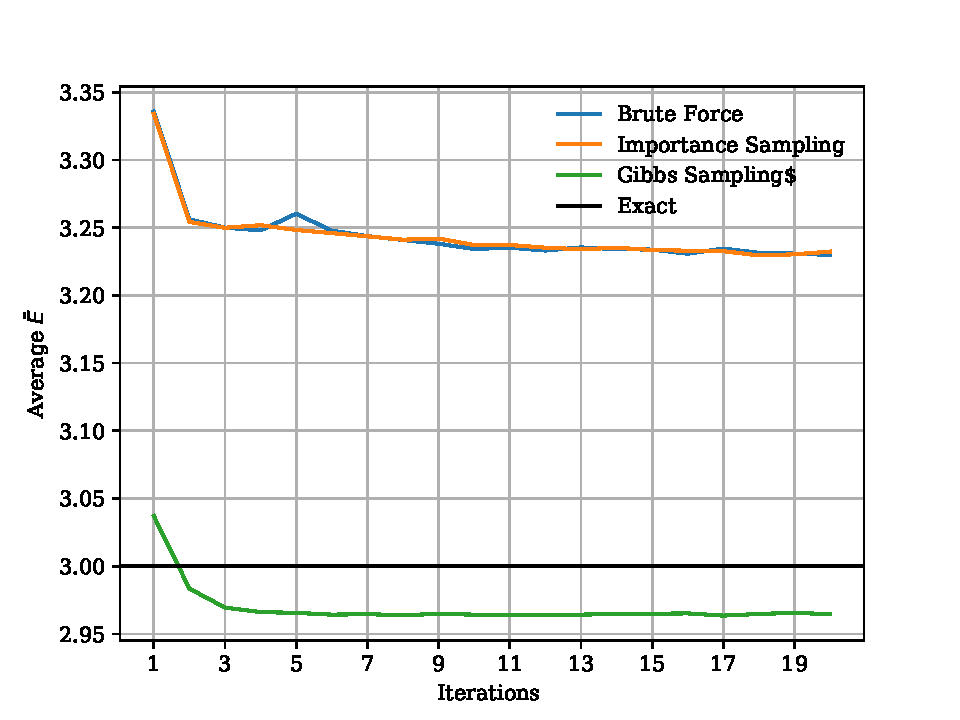
\includegraphics[scale=0.8]{../Results/sim_12/training_interacting.pdf} 
        \caption{energy}
        \label{fig:energy}   
\end{figure}  


\begin{figure}[!h]
        \centering 
         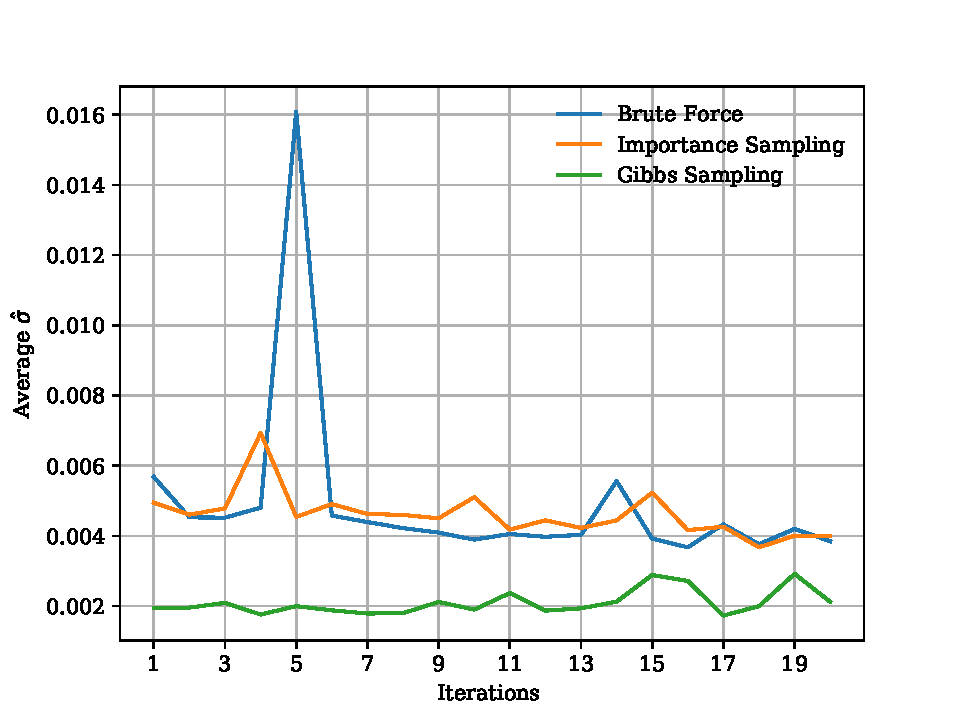
\includegraphics[scale=0.8]{../Results/sim_12/error_interacting.pdf} 
        \caption{error }
        \label{fig:inter_error}   
\end{figure}  

\begin{figure}[!h]
        \centering 
         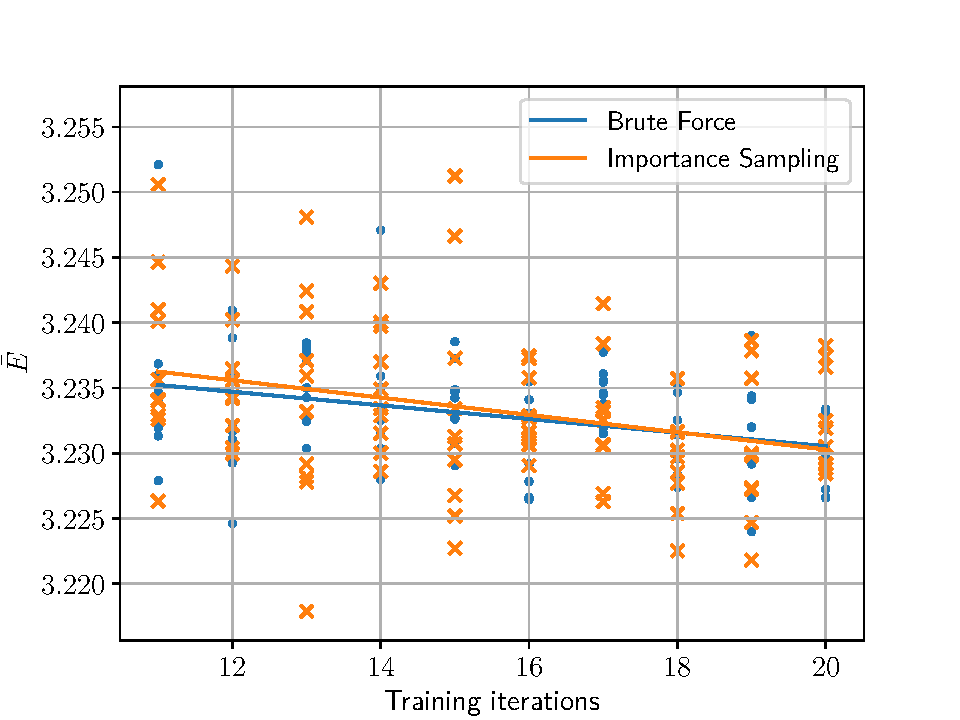
\includegraphics[scale=0.8]{../Results/sim_12/regression/Regression_BF_IS.pdf} 
        \caption{Brute Force \& Importance Sampling:  reg }
        \label{fig:reg_BFIS}   
\end{figure}  


\begin{figure}[!h]
        \centering 
         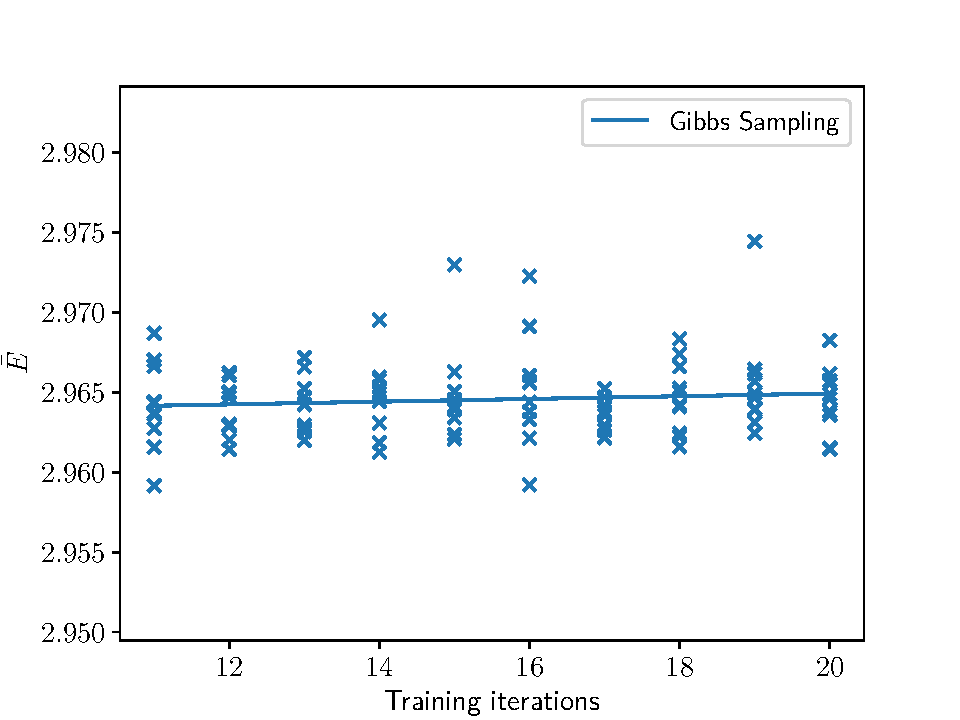
\includegraphics[scale=0.8]{../Results/sim_12/regression/Regression_GS.pdf} 
        \caption{Gibbs Sampling:  reg }
        \label{fig:reg_GS}   
\end{figure}  


\begin{table}[h!]
\begin{center}
\begin{tabular}{lll}
\hline
Method & Regression coefficient & Predicted iteration for $\bar E=3.0$  \\
\hline
BF &  $ -5 \times 10^{ -4 } $ & $ 462 $  \\
IS &  $ -7 \times 10^{ -4 } $ & $ 367 $  \\
GS &  $ 9 \times 10^{ -5 } $ & $433 $  \\
\hline
\end{tabular}
\end{center}
\caption{Comparison of VMC methods: Linear Regression fit}
\label{table:reg}
\end{table}

\subsection{Validity of results}
When determining the suitability of $l$ and $\Delta t$ I did not document the produced $\bar E$, as this would not have been feasible at that stage of the research (having not evaluated the training regime). This means that $l=1.0$ and $\Delta t=2.0$ might not be the best suited values after all, as lower variance is no guarantee for correct energy by it self. Furthermore, as I did not test values higher than $\Delta t=2.0$, higher values of $\Delta t$ may give lower $\hat sigma$ still. 

\ref{table:BF_IS_eta} was produced using noise reducing averaging over $5$ optimization steps and $15$ experiments, with consistent standard errors of $\sigma \sim 10^{-8}$ to $\sim 10^{9}$. Optimally, I should have included the MSE of $\hat \sigma$, but in order to limit the amount of information, I chose not to. A more  in-depth study could be done by also looking into the variance of the error, yielding even more robust results.

Averaging over $10$ runs in the interacting case is not robust enough 
\section{Conclusions} \label{conclusions}
As all values of $(\Delta E)^2$ was $\sim 10^{-5}$ for IS, compared to $\sim 10^{-4}$ to $\sim 10^{-5}$ depending on $\eta$ for BF, I conclude that when using an RBM, BF is more sensitive than IS to the choice of learning rate w.r.t accuracy of energy estimates. I furthermore conclude that the effects of $\eta$  on $\hat \sigma$ is the same for both BF and IS, regardless of the value of $\Delta t$. 
When using the optimal $\eta$ values based on $(\Delta E)^2$ alone, BF and IS performed equally well, producing $(\Delta E)^2 \approx 8.7 \times 10^{-8}$ with $\hat \sigma = 7 \times 10^{-8}$, when averaged over 15 experiments.
 hadde jeg hatt mer tid ville jeg prøvd å undersøke sigma mere. Kanskje det finnes noe forskning på det, eller noe i en lrebok, evenutelt kan den nok også læres med litt matte!
I suspect (without any that this difference in $\hat \sigma$ is a consequence of only using $n=2$ hidden nodes.

should be treated like an ML problem, using gridearch. Results from interacting are only valid ensorfar as results from non-interacting carries over!
\bibliography{ref} \label{refer}
\bibliographystyle{plain}


\begin{appendices}
\section{Appendix 1.} \label{APP_1}
\subsection{Analytic expression for the local energy}
\begin{equation}
\begin{aligned}
E_L &=\frac{1}{ \Psi_{rbm}  }   \sum_{i=1}^{M} \left(  -\frac{1}{2} \nabla_i^2 + \frac{1}{2} \omega^2 X_i^2  \right) \Psi_{rbm} + \frac{1}{ \Psi_{rbm} }  \sum_{i<j}^P \frac{1}{r_{ij}}  \Psi_{rbm} \\
&=\frac{1}{\Psi_{rbm}}   \sum_{i=1}^{M} \left(  -\frac{1}{2} \nabla_i^2 \Psi_{rbm} \right) + \sum_{i=1}^{M} \frac{1}{2} \omega^2 X_i^2    +  \sum_{i<j}^P\frac{1}{r_{ij}}  
\end{aligned}
\end{equation}
And
\begin{equation}
\begin{aligned}
\frac{1}{\Psi_{rbm}}\nabla^2 \Psi_{rbm} &=  \frac{1}{\Psi_{rbm}}\nabla (\Psi_{rbm} \frac{1}{\Psi_{rbm}} \nabla \frac{1}{\Psi_{rbm}})\\
&= (\frac{1}{\Psi_{rbm}} \nabla \Psi_T) ^2 + \nabla (\frac{1}{\Psi_{rbm}}\nabla \Psi_{rbm})\\ 
&= (\nabla \ln \Psi_{rbm})^2 + \nabla^2 \ln \Psi_{rbm}
\end{aligned}
\end{equation}
So
\begin{equation}
\begin{aligned}
E_L
&= -\frac{1}{2}  \sum_{k=1}^{M} \left( \nabla \ln \Psi_{rbm})^2 + \nabla^2 \ln \Psi_{rbm} \right) + \sum_{k=1}^{M} \frac{1}{2} \omega^2X_i^2    +  \sum_{i<j}^P\frac{1}{r_{ij}}  \\
\label{eq:Appendix_1EL}
\end{aligned}
\end{equation}


First derivative:
\begin{equation}
\begin{aligned}
\frac{1}{\Psi_{rbm}} \nabla_k \Psi_{rbm} &= \nabla_k  \ln \Psi_{rbm} \\
&= \nabla_k  \big( \ln \frac{1}{Z}  -\sum_i^M \frac{(X_i - a_i)^2}{2\sigma^2} +  \sum_j^N \ln (1 + e^{ b_j + \sum_i^M \frac{X_i w_{ij}}{\sigma^2}}) \big) \\
&= 
  - \frac{(X_k - a_k)}{\sigma^2} + \sum_{j}^N w_{kj}\frac{\exp (b_j + \sum_i^M \frac{x_i w_{ij}}{\sigma^2})}{1 + e^{ b_j + \sum_i^M \frac{X_i w_{ij}}{\sigma^2}}}  \\
&= - \frac{(X_k - a_k)}{\sigma^2} + \sum_{j}^N \frac{w_{kj}}{\sigma^2}\frac{1}{1 + e^{-v(\bm X,j)}}
\end{aligned}
\label{eq:Appendix_1derivative}
\end{equation}

Second derivative:
\begin{equation}
\begin{aligned}
\nabla_k^2  \ln \Psi_{rbm} &= \nabla_k  \big( 
   - \frac{(X_k - a_k)}{\sigma^2} + \sum_{j}^N \frac{w_{kj}}{\sigma^2}\frac{1}{1 + e^{-b_j  -\sum_i^M \frac{X_i w_{ij}}{\sigma^2}}}  \big) \\
  &=
 - \frac{1}{\sigma^2} + \sum_{j}^N \frac{w_{kj}^2}{\sigma^4}\frac{e^{-v(\bm X,j)}}{ ( 1 + e^{-v(\bm X,j)} )^2}  
\end{aligned}
\end{equation}
or

\begin{equation}
\begin{aligned}
\nabla \ln \Psi_{rbm}
&= - \frac{(X_k - a_k)}{\sigma^2} + \sum_{j}^N \frac{w_{kj}}{\sigma^2} \text {logistic} ( -v(j) ) 
\end{aligned}
\label{eq:Appendix_1derivative_rw}
\end{equation}

and
\begin{equation}
\begin{aligned}
\nabla^2 \ln \Psi_{rbm}
  &=
 - \frac{1}{\sigma^2} + \sum_{j}^N \frac{w_{kj}^2}{\sigma^4}  \text {logistic}^2 ( -v(j) ) \exp(-v(j))
\end{aligned}
\label{eq:Appendix_2derivative_rw}
\end{equation}

Thus to compute $E_L$, one may use \eqref{eq:Appendix_1EL}, \eqref{eq:Appendix_1derivative_rw} and \eqref{eq:Appendix_2derivative_rw}.









\section{Appendix 2.} \label{APP_2}
\subsection{Derivatives w.r.t RBM parameters}
Where $\frac{\bar \Psi_{\beta}}{\Psi [\beta]} = \frac{1}{\Psi_T [\beta]}\frac{d \Psi[\beta]}{d \beta}$. For parameter $k$: $\frac{1}{\Psi_T}\frac{\partial \Psi_T}{\partial \beta_k}=\frac{\partial}{\partial \beta_k} \log \Psi_T$

for $\beta=\bm a$:
\begin{equation}
\begin{aligned}
\frac{\partial}{\partial a_k} \log \Psi_T = \frac{X_k-a_k}{\sigma^2}
\end{aligned}
\label{eq:Appendix2_grad_a}
\end{equation}

for $\beta=\bm b$:
\begin{equation}
\begin{aligned}
\frac{\partial}{\partial b_k} \log \Psi_T 
= 
  \frac{1}{1 + e^{-v(\bm X,k)}}
\end{aligned}
\label{eq:Appendix2_grad_b}
\end{equation}

for $\beta=\bm W$:
\begin{equation}
\begin{aligned}
\frac{\partial}{\partial W_{kl}} \log \Psi_T = 
  \frac{X_k e^{v(\bm X,l)} }{(1 + e^{v(\bm X,l)}) \sigma^2} =
  \frac{X_k} {(1 + e^{-v(\bm X,l)}) \sigma^2} 
\end{aligned}
\label{eq:Appendix2_grad_b}
\end{equation}


\section{Appendix 3.} \label{APP_3}
\subsection{Appendix 3: Local energy and parameter gradients for Gibbs sampling}
As the only parts of $\Psi_T$ that is traceable in $E_L$ for this system are the derivatives of $ln \Psi_T$, 
\begin{equation}
\begin{aligned}
\Psi_{T,Gibbs}=\sqrt{F_{RBM}(\bm X)}=\sqrt{\Psi_{rbm} }
\end{aligned}
\label{eq:wfgibs}
\end{equation}

Means that the expression for $E_L$ remains the same as before, with the exceptions

\begin{equation}
\begin{aligned}
\nabla \ln \Psi_{rbm} = \frac{1}{2} \nabla \ln \Psi_{rbm}
\end{aligned}
\end{equation}

and

\begin{equation}
\begin{aligned}
\nabla^2 \ln \Psi_{rbm} = \frac{1}{2} \nabla^2 \ln \Psi_{rbm}
\end{aligned}
\end{equation}

And similarly for the parameter gradients, specifically for parameter number $k$ of $\bm \beta$;

\begin{equation}
\begin{aligned}
 \frac{1}{\Psi_{T,Gibbs} }\frac{\partial \Psi_{T,Gibbs} }{\partial \beta_k}=\frac{1}{2}\frac{\partial}{\partial \beta_k} \log \Psi_{rbm}
\end{aligned}
\end{equation}

\section{Appendix 4.} \label{APP_3}
\subsection{Appendix 4: Testing step length $l$ and $\Delta t$}
 I averaged the standard error (using blocking) $\hat \sigma$ from 12 experiments. In each experiment, I used $8$ MC simulations with parameter optimization (learning rate $\eta =0.3$), with $2^{21}$ MC cycles with a $0.5$ burn-in factor, for the shown values of $l$ and $\Delta t$ in figures \ref{fig:app_4_BF} and  \ref{fig:app_4_IS}.
I found that $l=1.0$ and $\Delta t = 2.0$ gave the best results among the tested values.
\begin{figure}[!h]
        \centering 
         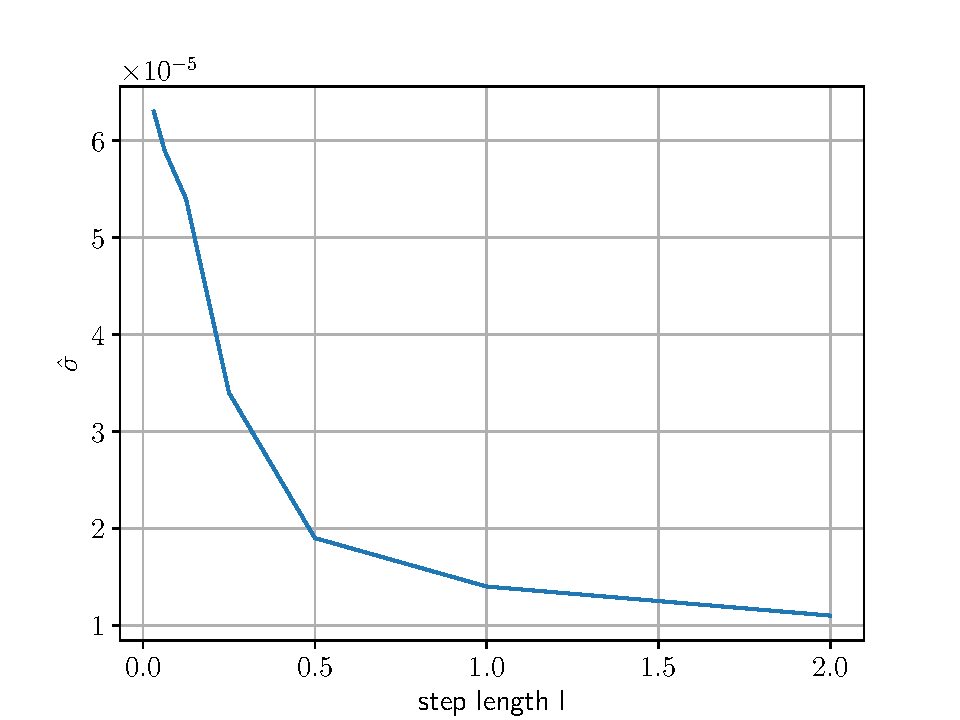
\includegraphics[scale=0.6]{../Results/sim_2/error.pdf} 
        \caption{Importance Sampling: $\hat \sigma$ as a function of $\Delta t$}
        \label{fig:app_4_IS}   
\end{figure}  

\begin{figure}[!h]
        \centering 
         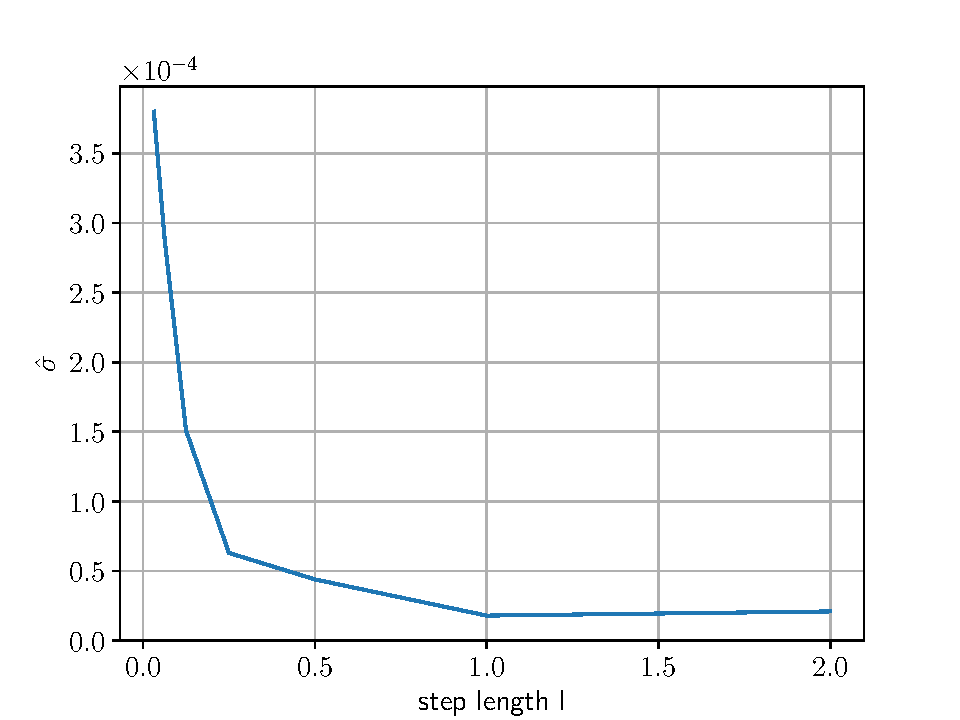
\includegraphics[scale=0.6]{../Results/sim_3/error.pdf} 
        \caption{Brute Force $\hat \sigma$ as a function of $l$}
        \label{fig:app_4_BF}   
\end{figure}  

\subsection{Appendix 4: Testing learning rate $\eta$}
\begin{figure}[!h]
        \centering 
         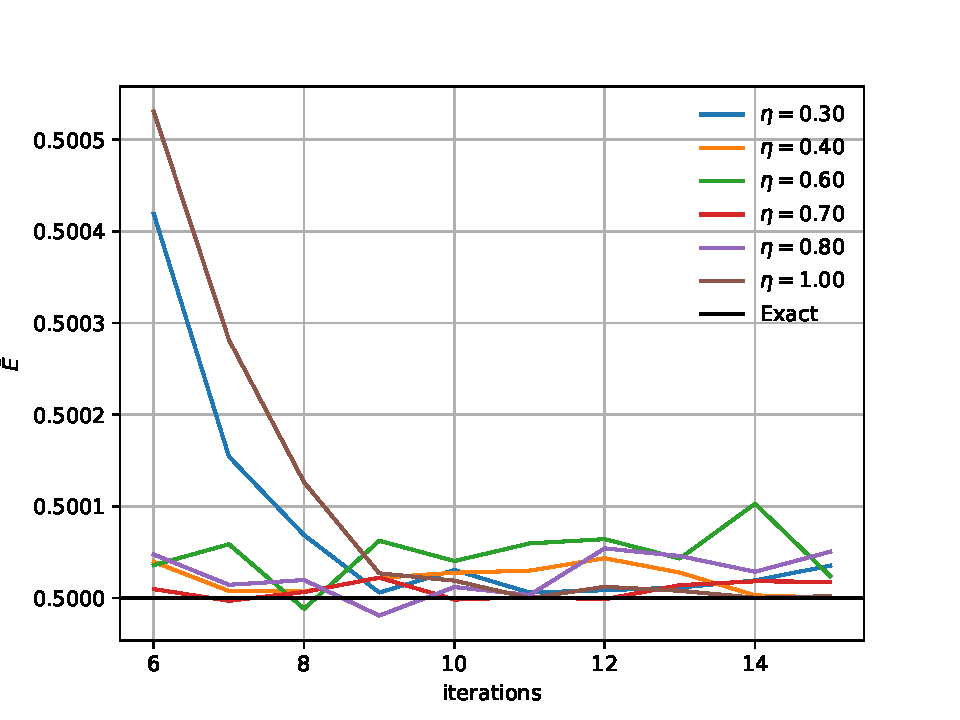
\includegraphics[scale=0.6]{../Results/sim_4/BF_eta.pdf} 
        \caption{Brute Force: $\bar E$ for different values of $\eta$ }
        \label{fig:training_BF}   
\end{figure}  

\begin{figure}[!h]
        \centering 
         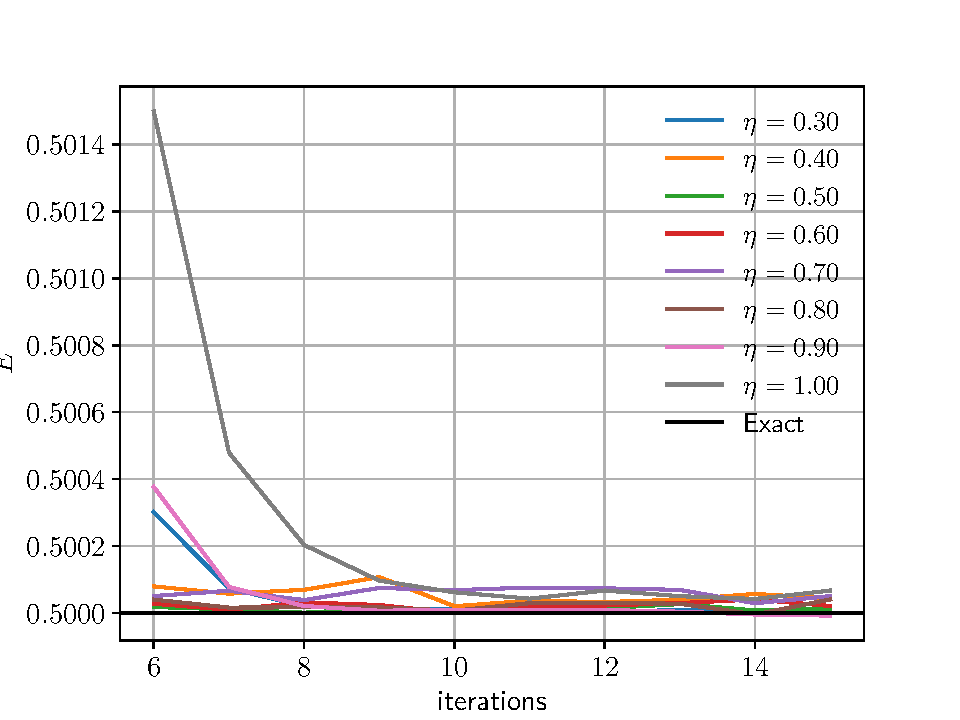
\includegraphics[scale=0.6]{../Results/sim_4/IS_eta.pdf} 
        \caption{Importance Sampling:  $\bar E$ for different values of $\eta$ }
        \label{fig:training_IS}   
\end{figure}  

\subsection{Appendix 4: Testing $\sigma$ and $\eta$ GS}
\begin{figure}[!h]
        \centering 
         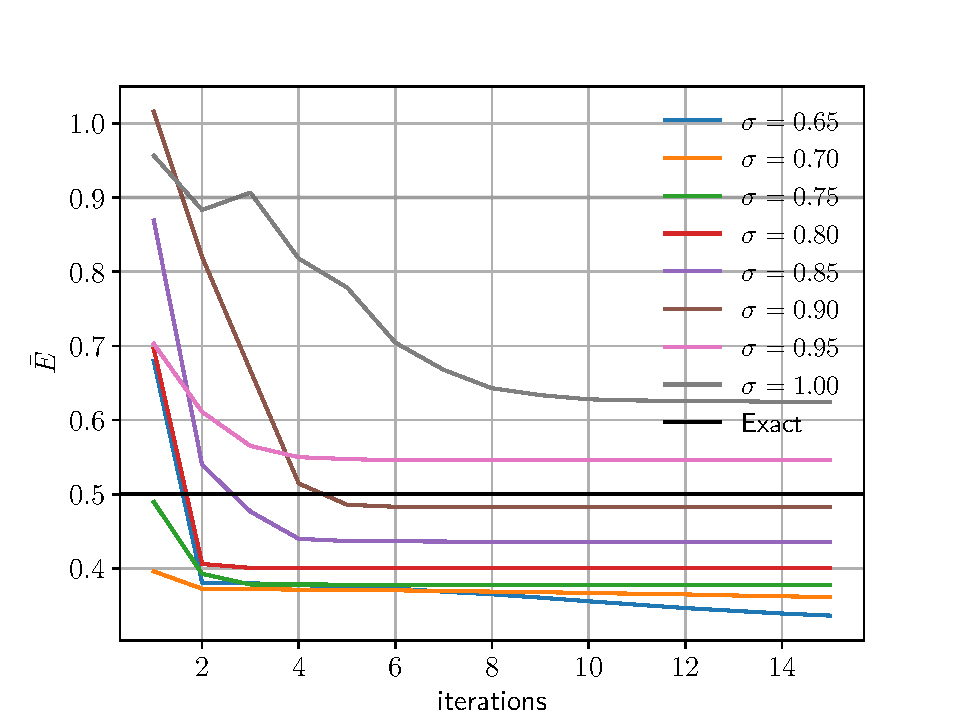
\includegraphics[scale=0.6]{../Results/sim_7/GS_initial.pdf} 
        \caption{Gibbs Sampling:  $\bar E$ for different values of $\sigma$ }
        \label{fig:GS_sigma_initial}   
\end{figure}  

\begin{figure}[!h]
        \centering 
         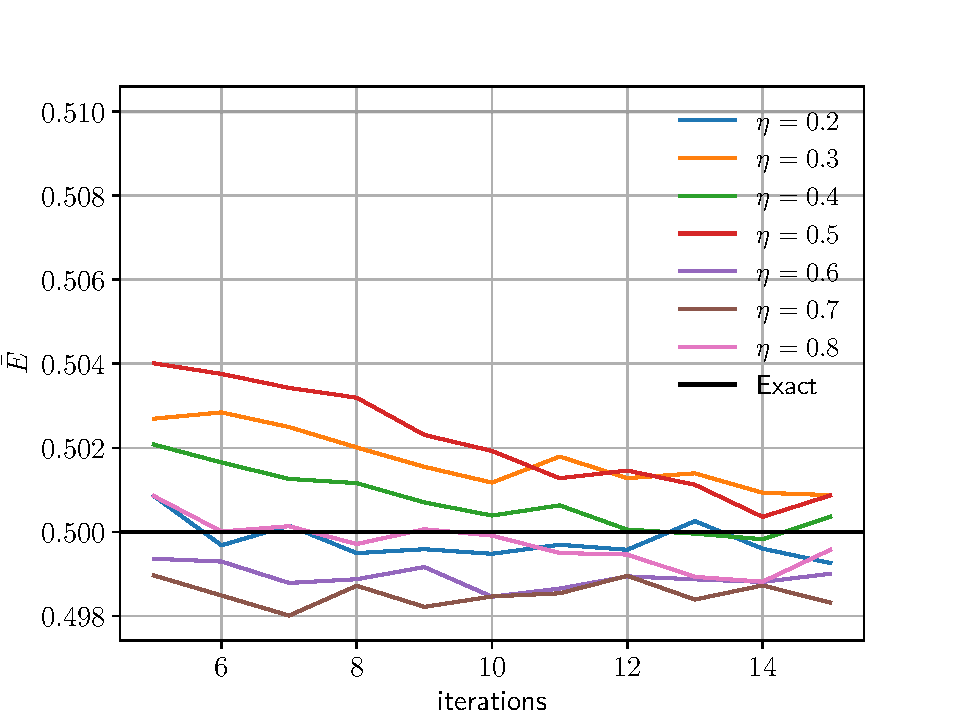
\includegraphics[scale=0.8]{../Results/sim_9/GS_eta.pdf} 
        \caption{Gibbs Sampling:  $\bar E$ for different values of $\eta$ }
        \label{fig:GS_eta}   
\end{figure}  

\end{appendices}
\end{document}